\documentclass[a4paper]{article}
\usepackage{graphicx} %Required for diagrams
\usepackage[bookmarks=true]{hyperref}
\usepackage{bookmark}%Required to do pdf bookmarking
\usepackage[margin=1.2in]{geometry}
\usepackage{float}
\usepackage{caption}
\usepackage{hyperref}%Required for referencing website pages
\usepackage[english]{babel}

\usepackage{graphicx}
\usepackage{dcolumn}
\usepackage[table]{xcolor}

\title{User Manual}
\author{Baobab Team}

\begin{document}
\newpage

\begin{titlepage}

\begin{center}


\includegraphics[width=400px]{pictures/logo.jpg}
\vspace{0.5 cm}
\begin{flushright} \large
\begin{tabular}{lr}
\vspace{1 cm}
\LARGE\textbf{Document:}Sprint Report 6\\

\vspace{1 cm}
\LARGE\textbf{Project:} Group Chat For Linphone (Agile DO-178)\\
\vspace{1 cm}
\LARGE\textbf{Advisor:} Kobus Coetzee\\
\vspace{1 cm}
\LARGE\textbf{Sponsors:} Nanoteq \& Department of Computer Science, UP\\
\vspace{1 cm}
\LARGE\textbf{Date: }\today\\
\end{tabular}
\end{flushright}

\centering 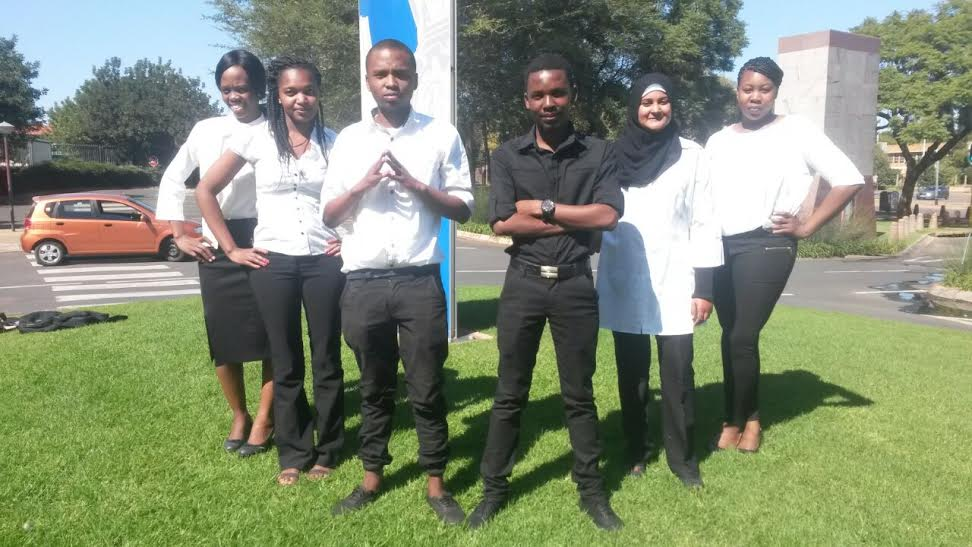
\includegraphics[width=350px]{pictures/Team.jpg}

Patience Mtsweni, Lerato Molokomme, Tsepo Ntsaba, Mpedi Mello, Lutfiyya Razak, Ephiphania Munava\\


\end{center}
\end{titlepage}
\newpage

\section{Introduction}
This user manual provides instructional support and guidance to help the users who use Linphone-android. The manual focuses on system configuration, installation, using the system, troubleshooting, etc.

\section{General Information}


\subsection{Project Details}

%Lerato edit here - System name and the names and/or affiliation of all stakeholders.
\setlength{\arrayrulewidth}{0.5mm}
\setlength{\tabcolsep}{12pt}
\renewcommand{\arraystretch}{2} 
\begin{tabular}{ |p{3cm}|p{3cm}|p{3cm}|  }
\hline
\rowcolor{lightgray}\multicolumn{2}{|c|}{System name affiliation of all stakeholders} \\
\hline
System name & Linphone Group Chat \\
\hline
Stakeholder & Kobus Coetzee \\
\hline
Scrum master  & Potego Mello\\ \hline 
Client representative  & Patience Mtsweni\\ \hline 
UX developer  & Lutfiyya Razak and Lerato Molokomme\\ \hline 
Backend developer  & Ephiphania Munava and Potego Mello\\ \hline 
Crypto developer  & Tsepo Ntsaba \\ \hline 
CI / CD support  & Patience Mtsweni \\ 
\hline
\end{tabular}

\subsection{System Overview}

The system we are working on is called Linphone. We are are adding additional functionality to an already existing project. The main aim of the functionality we are developing in the Linphone project is to allow a group of users to be able to communicate or exchange messages with each other. \\
This functionality is achieved by creating a group chat were there will be an interface that allows those messages to be exchanged and viewed. A  participant can send messages and pictures to a group, send voice recordings,update the group picture and change the  group name. \\
A participant can become an administrator in the group -  usually this is the person who creates the group ,who is 
responsible for adding and  removing other participants.\\


\subsection{System Configuration}

%Ephiphania Edit Here
\subsubsection{Equipment}
An Android phone is a smartphone that runs on Google's open-source Android operating system. There are a number of different manufacturers that make Android phones, namely HUAWEI, LG, ASUS, acer, Virgin mobile, Samsung, Motorola, Sony and many more.\\

\begin{center}
\begin{figure}[h]
\centering

\includegraphics[width=0.7\linewidth]{./pictures/android.jpg}
\caption{\label{fig:Agile}Android Phones.}
\end{figure}
\end{center}

\subsubsection{Network}
The linphone application requires registration to a SIP provider before you can operate it. The provider ensures that you have a SIP address which is a Uniform Resource Identifier also known as a URI which is represented in the form user@domain.tld. \\


\begin{center}
\begin{figure}[h]
\centering
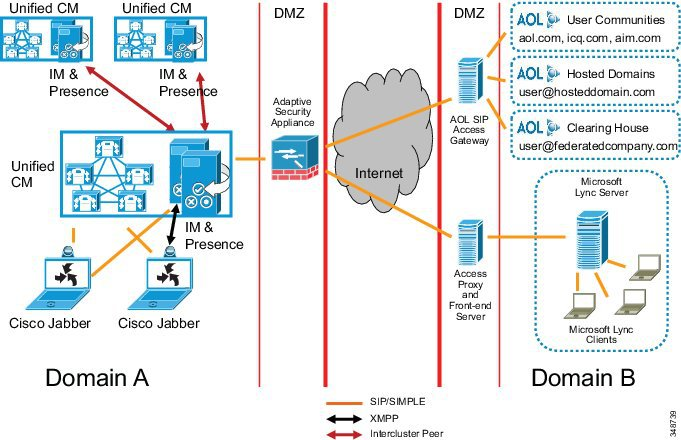
\includegraphics[width=0.7\linewidth]{./pictures/sip.jpg}
\caption{\label{fig:Agile}SIP Protocol.}
\end{figure}
\end{center}

Linphone.org hosts a free SIP service which allows users to make audio or video calls using SIP addresses under the domain sip.linphone.org. \\
When creating your sip address like sip:baobab@sip.linphone.org you simple use the form provided on http://www.linphone.org/free-sip-service.html and your friends can communicate with you by simply making use of the sip address.


\newpage
\begin{center}
\begin{figure}[h]
\centering
\includegraphics[width=0.4\linewidth]{./pictures/LinphoneSip.jpg}
\caption{\label{fig:Agile}Linphone SIP Registration.}
\end{figure}
\end{center}


\subsection{Installation}
\begin{itemize}
\item Turn on your Android Smartphone and click on the Google Play icon to launch Google Play.
\item Tap the “Search” button in the upper right corner and type “Linphone”
\item From the result list tap the result with the title “Linphone Video” to expand it
\item Tap the “Install” button, Linphone for Android will be downloaded and the installation procedure will begin
\item Confirm that you accept the Linphone application rights on the screen that will be appear on your Smartphone by tapping “Accept”. When the file installation is done tap “Open”.
\item Press “Agree” when the License Agreement appears on your screen to finalize the install and start Linphone for Android.
\end{itemize}

\subsection{Getting started}
%Patience Edit Here
Our system is a group chat which is part of an existing Instant Messaging Application called Linphone. Therefore, for a you to access our system you need to have downloaded the application onto your android mobile device. To do this,  refer to section 2.4 (Installation) and follow the instructions as specified there. After installing Linphone onto your phone, you need to register in order to be able to use the application.
You can register by following these steps:
\begin{itemize}
\item Click on the "Settings" button on the bottom right corner. After clicking it, the following screen will appear:
\end{itemize}

%\begin{center}
\begin{figure}[h]
\centering
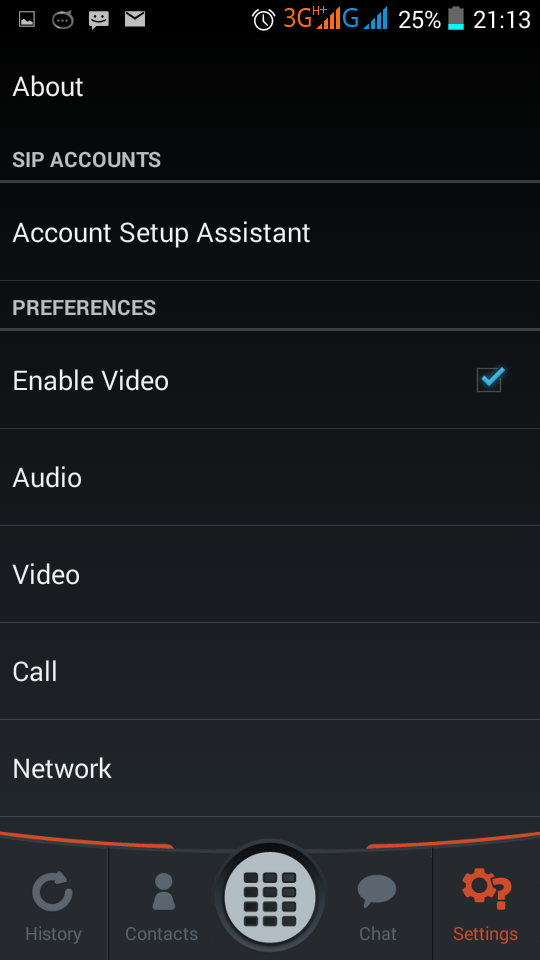
\includegraphics[scale=0.30, width=40mm]{./pictures/settings.png}
\caption{\label{fig:Agile}Settings}
\end{figure}
%\end{center}

\begin{itemize}
\item Click/press "Account Setup Assistant".  After clicking it, you will see the screen as shown by figure 4, in this screen click "Let's go" to go to the next screen.
\end{itemize}

%\begin{center}
\begin{figure}[h]
\centering

\includegraphics[scale=0.30, width=40mm]{./pictures/welcome.png}
\caption{\label{fig:Agile}Account Setup Assistant}
\end{figure}
%\end{center}

\begin{itemize}
\item Next, click on any  one of the following that are applicable to you, for example, if you do not have a linphone.org account, you should click/press "Create an account on linphone.org". The following screen will appear, when it does, fill your details and click "create".
\end{itemize}

%\begin{center}
\begin{figure}[h]
\centering
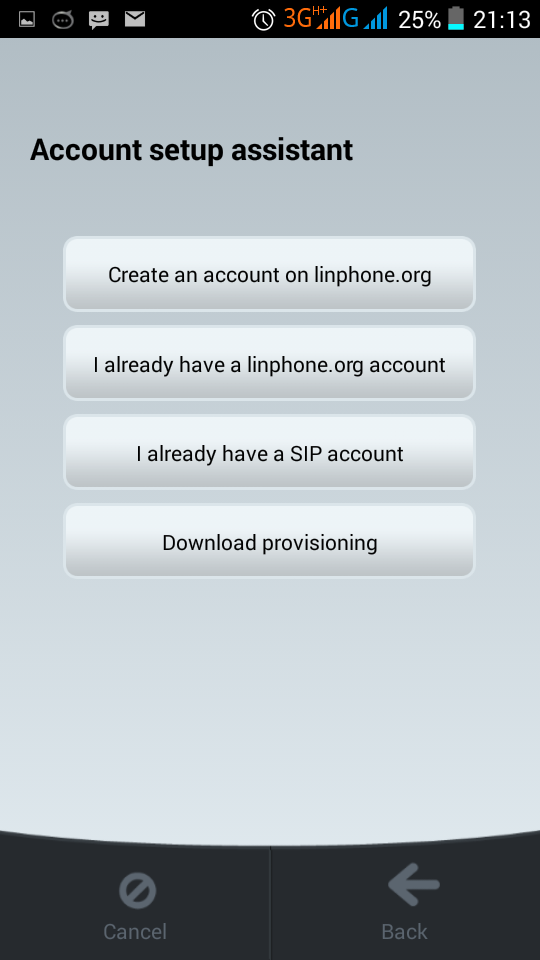
\includegraphics[scale=0.30, width=40mm]{./pictures/options.png}
\caption{\label{fig:Agile}Create Account}
\end{figure}
%\end{center}

After following these steps, you will be registered and ready to use the application. (Note, that after registering you will need to verify your account by clicking on the link that will be in the e-mail sent by linphone.org to your email address).

Now that you are registered, follow these steps to access the group chat:

\begin{itemize}
\item Click/press "chat".
\end{itemize}

%\begin{center}
\begin{figure}[h]
\centering
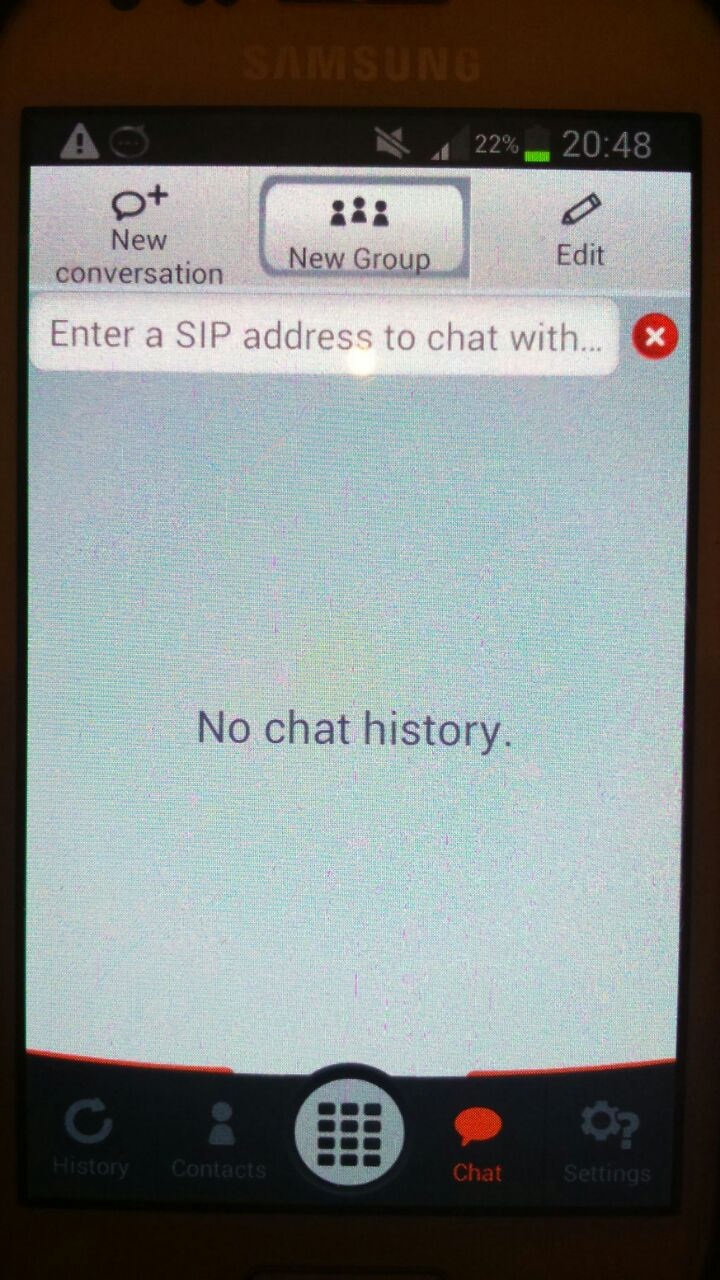
\includegraphics[scale=0.30, width=40mm]{./pictures/s1.jpg}
\caption{\label{fig:Agile}Chat Screen}
\end{figure}
%\end{center}

\begin{itemize}
\item Click/press "New Group". As shown at the top of figure 6. After clicking it, the following screen will appear:
\end{itemize}

%\begin{center}
\begin{figure}[h]
\centering
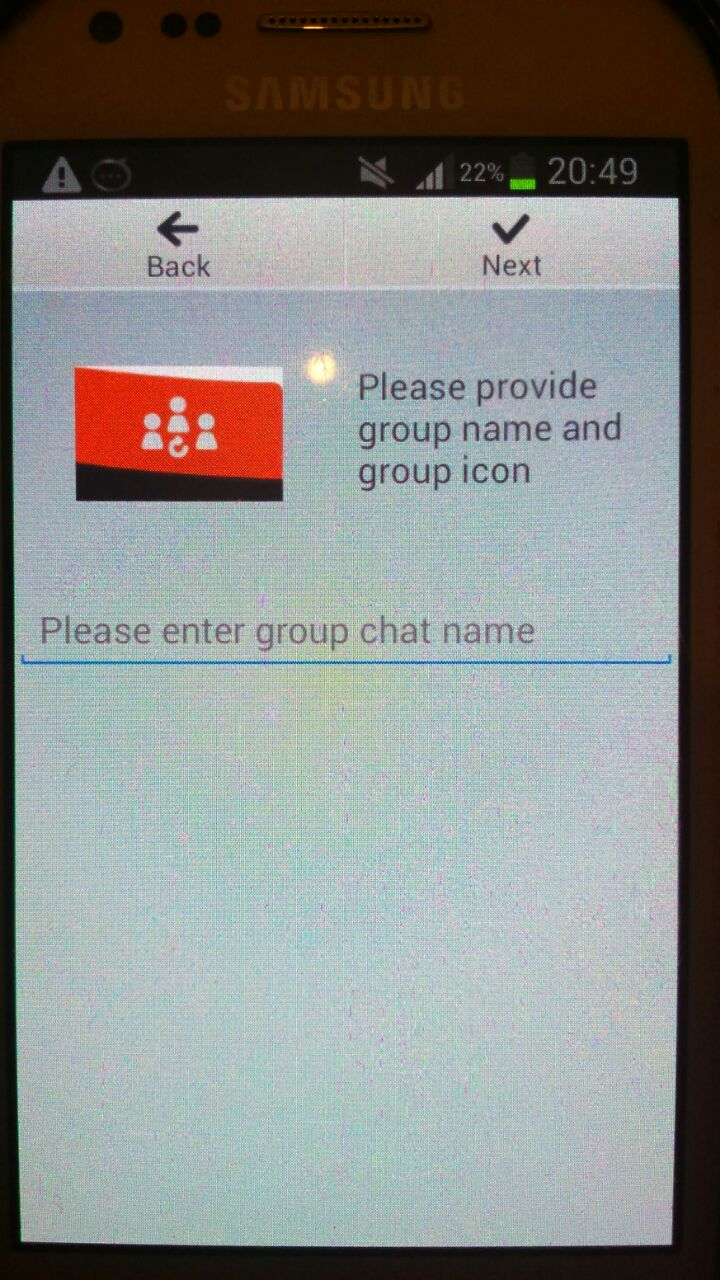
\includegraphics[scale=0.30, width=40mm]{./pictures/s2.jpg}
\caption{\label{fig:Agile}New Group Screen}
\end{figure}
%\end{center}

\begin{itemize}
\item Enter your group name in the space provided and choose an icon/profile picture(optional), as shown in figure 7, to proceed to next screen. 
\end{itemize}

\begin{itemize}
\item Click "next" on figure 7 to go to the following screen:
\end{itemize}

%\begin{center}
\begin{figure}[h]
\centering
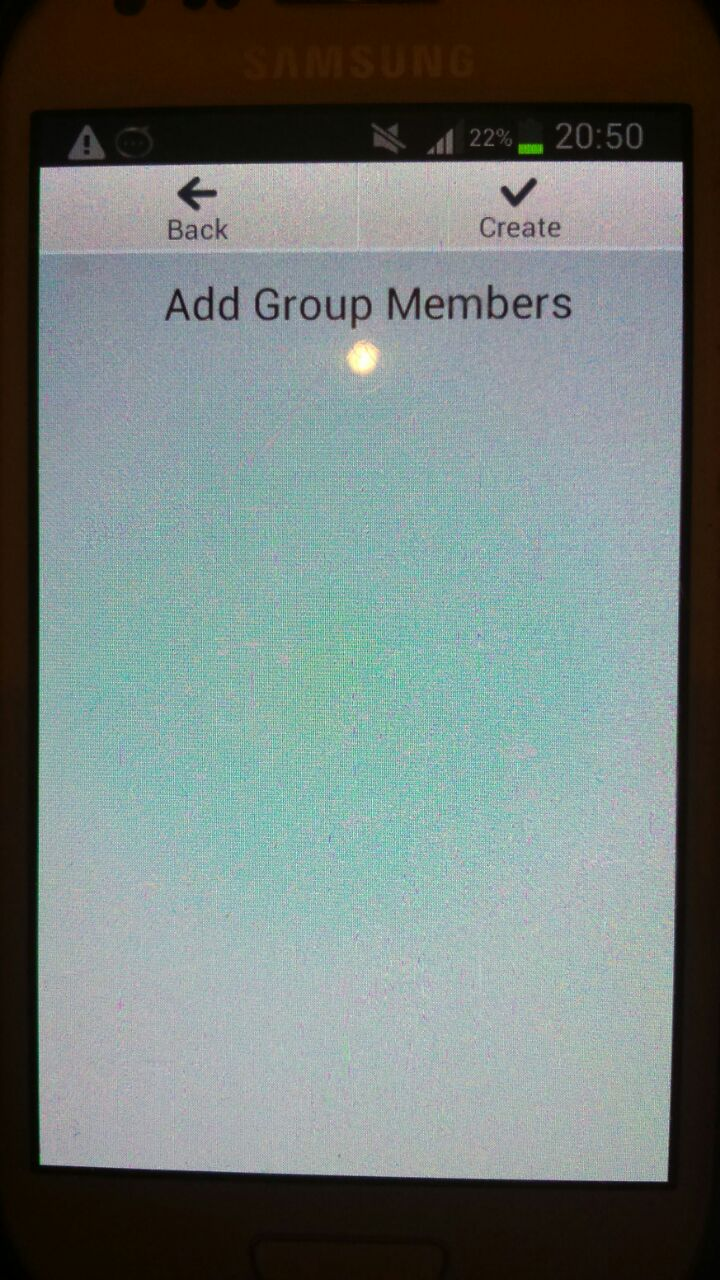
\includegraphics[scale=0.30, width=40mm]{./pictures/s3.jpg}
\caption{\label{fig:Agile}Chatroom screen}
\end{figure}
%\end{center}




\newpage
\subsection{Using the system}
%Potego Edit Here

\subsection{System Configuration}
%Tsepo Edit Here

\end{document}
